%%%%%%%%%%%%%%%%%%%%%%%%%%%%%%%%%%%%%%%%%
% Beamer Presentation
% LaTeX Template
% Version 1.0 (10/11/12)
%
% This template has been downloaded from:
% http://www.LaTeXTemplates.com
%
% License:
% CC BY-NC-SA 3.0 (http://creativecommons.org/licenses/by-nc-sa/3.0/)
%
%%%%%%%%%%%%%%%%%%%%%%%%%%%%%%%%%%%%%%%%%

%-------------------------------------------------------------------------------
%	PACKAGES AND THEMES
%-------------------------------------------------------------------------------

\documentclass[xcolor=table]{beamer}
\usepackage{graphicx}
\usepackage{tikz}
\usepackage{listings}
\usepackage{multicol}
\usepackage{amsmath}
\usepackage{amssymb}
\usepackage{amsthm}

\usepackage{lmodern}
\usepackage[T1]{fontenc}

\definecolor{applegreen}{rgb}{0.55, 0.71, 0.0}
\definecolor{blue(ncs)}{rgb}{0.0, 0.45, 0.60}
\definecolor{burgundy}{rgb}{0.5, 0.0, 0.13}

\definecolor{cadet}{rgb}{0.33, 0.41, 0.47}
\definecolor{airforceblue}{rgb}{0.36, 0.54, 0.66}

\lstdefinestyle{C}{
  language=C,
  emptylines=1,
  breaklines=true,
  basicstyle=\ttfamily\color{black},
  identifierstyle=\ttfamily,
  keywordstyle=\color[rgb]{0.0, 0.0, 1.0},
  stringstyle=\color[rgb]{1.0, 0.0, 0.0},
  commentstyle=\color{gray}\slshape,
}

\mode<presentation> {

\usetheme{CambridgeUS}

\usecolortheme{wolverine}

\definecolor{gold}{HTML}{D4A017}
\definecolor{darkgold}{HTML}{B7950B}

\setbeamercolor{palette primary}{bg=cadet,fg=white}
\setbeamercolor{palette secondary}{bg=airforceblue,fg=white}
\setbeamercolor{palette tertiary}{bg=black,fg=white}
\setbeamercolor{palette quaternary}{bg=cadet,fg=white}

\setbeamercolor{frametitle}{bg=airforceblue,fg=white}

\setbeamercolor{section number projected}{bg=black,fg=cadet}
\setbeamercolor{item}{fg=black,bg=cadet}

\setbeamertemplate{page number in head/foot}[framenumber]
}

\usepackage{graphicx} % Allows including images
\usepackage{booktabs} % Allows the use of \toprule, \midrule and \bottomrule in tables

%-------------------------------------------------------------------------------
%	TITLE PAGE
%-------------------------------------------------------------------------------

\title[Preconditioning High-Order FEM]{Preconditioning Matrix-Free High-Order\\Finite Element Operators} % The short title appears at the bottom of every slide, the full title is only on the title page

\author[Jeremy L Thompson]{Jeremy L Thompson} % Your name
\institute[CU Boulder] % Your institution as it will appear on the bottom of every slide, may be shorthand to save space
{University of Colorado Boulder \\ % Your institution for the title page
\medskip
\textit{jeremy.thompson@colorado.edu} % Your email address
}
\date{Apr 13, 2020} % Date, can be changed to a custom date

\begin{document}

\begin{frame}
\titlepage % Print the title page as the first slide
\end{frame}

%-------------------------------------------------------------------------------

\begin{frame}
\begin{center}
\frametitle{Overview}

Finite element methods with global sparse matrices are not\\
adequate for exascale solid mechanics problems\\~\\

High-order matrix-free operators offer superior performance\\
with respect to FLOPs and memory transfer for a matrix-vector product\\~\\


$p$-multigrid preconditioners are effective for matrix-free FEM\\
and new to Neo-Hookean hyperelasticity at finite strain\\~\\

Further research required for matrix-free smoothers,\\
BDDC smoothers, subdomain solvers, and split preconditioners

\end{center}
\end{frame}
 
%-------------------------------------------------------------------------------

\begin{frame}
\frametitle{Overview} % Table of contents slide, comment this block out to remove it
\tableofcontents % Throughout your presentation, if you choose to use \section{} and \subsection{} commands, these will automatically be printed on this slide as an overview of your presentation
\end{frame}

%-------------------------------------------------------------------------------
%	PRESENTATION SLIDES
%-------------------------------------------------------------------------------

%-------------------------------------------------------------------------------
\section{Introduction}
%-------------------------------------------------------------------------------

\begin{frame}
\begin{center}
\frametitle{Center for Efficient Exascale Discretizations}

\begin{flushleft}
DoE exascale co-design center\\

\end{flushleft}

\begin{itemize}

\item Design discretization algorithms for exascale hardware that deliver significant performance gain over low order methods\\~\\

\item Collaborate with hardware vendors and software projects for exascale hardware and software stack\\~\\

\item Provide efficient and user-friendly unstructured PDE discretization component for exascale software ecosystem

\end{itemize}

\end{center}
\end{frame}

%-------------------------------------------------------------------------------
\section{Hardware Constraints}
%-------------------------------------------------------------------------------

\begin{frame}
\begin{center}
\frametitle{Hardware Limitations}

\begin{multicols}{2}

\includegraphics[width=.99\linewidth]{../img/peakFlopsAndBandwidthTall}

\begin{itemize}

\item Memory and network bandwidth improvements lag behind FLOPs\\~\\

\item Trend is consistent across manufacturers\\~\\

\item Similar developments for different systems over 30 years

\end{itemize}

\end{multicols}

\end{center}
\end{frame}

%-------------------------------------------------------------------------------

\begin{frame}
\begin{center}
\frametitle{FLOPs vs Bandwidth}

\begin{multicols}{2}

\begin{itemize}

\item Memory bound applications can't reach peak FLOPs\\~\\

\item Network communication also a well known scaling issue\\~\\

\item GPU computation also requires host-device communication

\end{itemize}

\vfill\null
\columnbreak

\includegraphics[width=.95\linewidth]{../img/peakRatioTall}

\end{multicols}

\end{center}
\end{frame}

%-------------------------------------------------------------------------------

\begin{frame}
\begin{center}
\frametitle{Benchmarks}

\begin{tabular}{l | c | c | c}
\rowcolor{airforceblue}
\textcolor{white}{System} & \textcolor{white}{HPL TFLOPs} & \textcolor{white}{HPCG TFLOPs} & \textcolor{white}{\% HPL} \\
\hline
\rowcolor{cadet!30}
Summit & $148,600.0$ & $2,925.75$ & $1.97$\\
Sierra & $94,640.0$ & $1,795.67$ & $1.90$\\
\rowcolor{cadet!30}
Trinity & $20,158.7$ & $546.12$ & $2.71$\\
ABCI & $19.880.0$ & $508.85$ & $2.56$\\
\rowcolor{cadet!30}
Piz Daint & $21,230.0$ & $496.98$ & $2.34$
\end{tabular}

~\\~\\

\begin{itemize}

\item Applications often can't match HPL performance\\~\\

\item Memory and network bandwidth limit application code\\~\\

\item Matrix-free formulations can target this disparity

\end{itemize}

\end{center}
\end{frame}

%-------------------------------------------------------------------------------
\section{Matrix-Free Finite Elements}
%-------------------------------------------------------------------------------

\begin{frame}
\begin{center}
\frametitle{Finite Element Operators}

PDE Weak Form:\\~\\

find $u \in V$ such that for all $v \in V$
\[
\langle v, u \rangle = \int_{\Omega} v \cdot f_0 \left( u, \nabla u \right) + \nabla v : f_1 \left( u, \nabla u \right) = 0
\]\\~\\~\\

\begin{itemize}

\item Weak form of PDEs are linear in the test functions\\~\\

\item PDE need not be linear for this general form\\~\\

\item Boundary integrals introduce similar terms

\end{itemize}

\end{center}
\end{frame}

%-------------------------------------------------------------------------------

\begin{frame}
\begin{center}
\frametitle{Galerkin System}

Galerkin System:\\

\[
  \sum_e \mathcal{E}^T \left[ \left( \mathbf{B}^e \right)^T \mathbf{W}^e \Lambda \left( f_0 \left( u^e, \nabla u^e \right) \right) + \sum_{i = 0}^{d - 1} \left( \mathbf{D}_i^e \right)^T \mathbf{W}^e \Lambda \left( f_1 \left( u^e, \nabla u^e \right) \right) \right] = 0
\]
where $u^e = \mathbf{B}^e \mathcal{E}^e u$ and $\nabla u^e = \lbrace \mathbf{D}_i^e \mathcal{E}^e u \rbrace_{i = 0}^{d - 1}$\\~\\~\\

\begin{itemize}

\item $\mathcal{E}^e$ - element restriction operator\\~\\

\item $\mathbf{B}^e$/$\mathbf{D}^e$ - interpolation/derivatives from DoFs to quadrature points\\~\\

\item $W^e$ - element quadrature weights, with geometric deformation\\~\\

\item $\Lambda$ - pointwise multiplication at quadrature points

\end{itemize}

\end{center}
\end{frame}

%-------------------------------------------------------------------------------

\begin{frame}
\begin{center}
\frametitle{Galerkin System}

Galerkin System:\\

\[
  \sum_e \mathcal{E}^T \left[ \left( \mathbf{B}^e \right)^T \mathbf{W}^e \Lambda \left( f_0 \left( u^e, \nabla u^e \right) \right) + \sum_{i = 0}^{d - 1} \left( \mathbf{D}_i^e \right)^T \mathbf{W}^e \Lambda \left( f_1 \left( u^e, \nabla u^e \right) \right) \right] = 0
\]
where $u^e = \mathbf{B}^e \mathcal{E}^e u$ and $\nabla u^e = \lbrace \mathbf{D}_i^e \mathcal{E}^e u \rbrace_{i = 0}^{d - 1}$\\~\\~\\

\begin{itemize}

\item Can express non-linear residual evaluators or linear Jacobians\\~\\

\item Notice no explicit mesh structure or homogeneity assumed\\~\\

\item Face integrals introduce similar terms

\end{itemize}

\end{center}
\end{frame}

%-------------------------------------------------------------------------------

\begin{frame}
\begin{center}
\frametitle{Practical Implementation}

\includegraphics[width=.99\linewidth]{../img/libCEEDAPI}

\end{center}
\end{frame}

%-------------------------------------------------------------------------------

\begin{frame}
\begin{center}
\frametitle{Efficient Implementation}

Galerkin System:\\

\[
  {\color{burgundy} A} = \sum_e {\color{gray}\mathcal{E}}^T \left[ \left( {\color{blue(ncs)} \mathbf{B}^e} \right)^T {\color{applegreen} \mathbf{W}^e} \Lambda \left( {\color{applegreen} f_0} \left( u^e, \nabla u^e \right) \right) + \sum_{i = 0}^{d - 1} \left( {\color{blue(ncs)} \mathbf{D}_i^e} \right)^T {\color{applegreen} \mathbf{W}^e} \Lambda \left( {\color{applegreen} f_1} \left( u^e, \nabla u^e \right) \right) \right]
\]
where $u^e = {\color{blue(ncs)}\mathbf{B}^e} {\color{gray}\mathcal{E}^e} u$ and $\nabla u^e = \lbrace {\color{blue(ncs)}\mathbf{D}_i^e} {\color{gray}\mathcal{E}^e} u \rbrace_{i = 0}^{d - 1}$\\~\\~\\

\begin{itemize}

\item Same framework for assembly of sparse matrices for finite elements\\~\\

\item Eschewing assembly allows optimizations and parallelism

\end{itemize}

\end{center}
\end{frame}

%-------------------------------------------------------------------------------

\begin{frame}
\begin{center}
\frametitle{Tensor Contractions}

3D Tensor Basis Operators:

\[
\begin{array}{c}
{\color{blue(ncs)}\mathbf{B}  } = B \otimes B \otimes B \hspace{10mm}
{\color{blue(ncs)}\mathbf{D}_0} = D \otimes B \otimes B\\~\\
{\color{blue(ncs)}\mathbf{D}_1} = B \otimes D \otimes B \hspace{10mm}
{\color{blue(ncs)}\mathbf{D}_2} = B \otimes B \otimes D\\~\\
{\color{applegreen}\mathbf{W} } = W \otimes W \otimes W
\end{array}
\]

\begin{itemize}

\item $B$, $D$, $W$ are 1D basis and quadrature weight matrices\\~\\

\item Basis evaluation is computationally expensive\\~\\

\item Tensor product elements allow efficient basis operations\\~\\

\end{itemize}

\end{center}
\end{frame}

%-------------------------------------------------------------------------------

\begin{frame}
\begin{center}
\frametitle{Single Element Performance}

\begin{multicols}{2}

\includegraphics[width=.99\linewidth]{../img/assembledVsMatrixFreeTall}

\begin{itemize}

\item Test operator: $\left( \nabla^2 - \alpha^2 \right) u$\\~\\

\item Assembled:\\ FLOPs and memory per DoF scale cubicly\\~\\

\item Matrix-Free:\\ FLOPs per DoF scale linearly, memory constant

\end{itemize}

\end{multicols}

\end{center}
\end{frame}

%-------------------------------------------------------------------------------

\begin{frame}
\begin{center}
\frametitle{Single Element Performance}

\begin{multicols}{2}

\begin{itemize}

\item Matrix-free implementation closer to hardware capabilities\\~\\

\item Performance gets better at higher order

\end{itemize}

~\\

\includegraphics[width=.5\linewidth]{../img/peakRatioTall}

\vfill\null
\columnbreak

\includegraphics[width=.95\linewidth]{../img/assembledVsMatrixFreeBalanceTall}

\end{multicols}

\end{center}
\end{frame}

%-------------------------------------------------------------------------------
\section{Hyperelasticity}
%-------------------------------------------------------------------------------

\begin{frame}
\begin{center}
\frametitle{Hyperelasticity}

Static balance of linear momentum at finite strain:
\[
- \nabla_X \cdot \boldsymbol{P} - \rho_0 \boldsymbol{g} = 0
\]

First Piola-Kirchhoff stress tensor:
\[
\boldsymbol{P} = \boldsymbol{F} \, \boldsymbol{S} \hspace{5mm} \boldsymbol{F} = \boldsymbol{I} + \nabla_X u
\]

\begin{itemize}

\item Hyperelasticity at finite strain near the incompressible regime\\~\\

\item Second Piola-Kirchhoff stress tensor $\boldsymbol{S}$ given by constitutive model\\~\\

\item Standard implementations struggle to scale on modern hardware

\end{itemize}

\end{center}
\end{frame}

%-------------------------------------------------------------------------------

\begin{frame}
\begin{center}
\frametitle{Neo-Hookean Hyperelasticity}

Neo-Hookean constitutive model:
\[
\boldsymbol{S} = \lambda \log \left( \lvert \boldsymbol{F} \rvert \right) \boldsymbol{C}^{-1} + 2 \mu \boldsymbol{C}^{-1} \boldsymbol{E}
\]

\begin{itemize}

\item In terms of:\\
  Right Cauchy-Green tensor $\boldsymbol{C} = \boldsymbol{F}^T \boldsymbol{F}$\\
  Green-Lagrange strain tensor $\boldsymbol{E} = \frac{1}{2} \left( \boldsymbol{C} - \boldsymbol{I} \right)$\\~\\

\item Lam{\'e} parameters:\\
  $\lambda = \frac{E \nu}{\left( 1 + \nu \right)\left( 1 - 2 \nu \right)}$ and
  $\mu = \frac{E}{2 \left( 1 + \nu \right)}$\\~\\

\item Convergence slow near incompressible limit: $\nu \rightarrow 0.5$

\end{itemize}

\end{center}
\end{frame}

%-------------------------------------------------------------------------------

\begin{frame}
\begin{center}
\frametitle{Test Case}

\begin{multicols}{2}

\includegraphics[width=.9\linewidth]{../img/deformBefore}

Before Deformation

\includegraphics[width=.9\linewidth]{../img/deformAfter}

After Deformation

\end{multicols}

\begin{itemize}

\item Deformation of rectangular or cylindrical beam\\~\\

\item 1 radian axial twist while translating opposite end

\end{itemize}

\end{center}
\end{frame}

%-------------------------------------------------------------------------------

\begin{frame}
\begin{center}
\frametitle{Self Convergence Study}

\begin{multicols}{2}

\includegraphics[width=.9\linewidth]{../img/convergeHRefine}

\includegraphics[width=.9\linewidth]{../img/convergePRefine}

\end{multicols}

\begin{itemize}

\item Error in strain energy under mesh refinement\\~\\

\item Currently there is an issue with the study for degree $3$ and $4$

\end{itemize}

\end{center}
\end{frame}

%-------------------------------------------------------------------------------
\section{Preconditioning}
%-------------------------------------------------------------------------------

\begin{frame}
\begin{center}
\frametitle{Preconditioners}

Left Preconditioning:

\[
\mathbf{A} x = b \hspace{5mm} \mathbf{\rightarrow} \hspace{5mm} \mathbf{M}^{-1} \mathbf{A} x = \mathbf{M}^{-1} x
\]
where $\mathbf{M}^{-1} \approx \mathbf{A}^{-1}$\\~\\

\begin{itemize}

\item Matrix-free operators require iterative solvers\\~\\

\item Preconditioning is required for efficient implementation\\~\\

\item Conjugate Gradient is a popular but restrictive iterative solver

\end{itemize}

\end{center}
\end{frame}

\subsection{$p$-multigrid}
%-------------------------------------------------------------------------------

\begin{frame}
\begin{center}
\frametitle{$p$-multigrid}

\begin{multicols}{2}

\includegraphics[width=.59\linewidth]{../img/quadraticShape}

\includegraphics[width=.59\linewidth]{../img/linearShape}

$p$-multigrid is ideal for matrix-free on unstructured meshes\\~\\

\begin{itemize}

\item Multigrid provides mesh independent convergence\\~\\

\item Algebraic multigrid requires matrix assembly\\~\\

\item $h$-multigrid difficult on unstructured/mixed meshes

\end{itemize}

\end{multicols}

\end{center}
\end{frame}

%-------------------------------------------------------------------------------

\begin{frame}
\begin{center}
\frametitle{V-Cycle}

3 level multigrid example\\
~\\

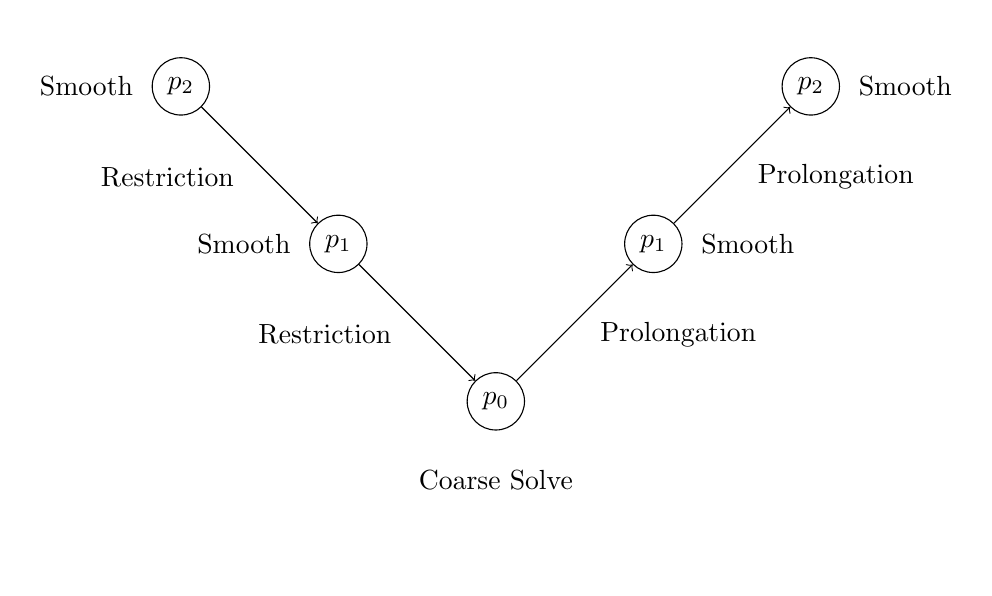
\begin{tikzpicture}
\node[shape=circle,draw=black] (A) at (0,0) {$p_2$};
\node[shape=circle] (Al) at (-1.2,0) {Smooth};
\node[shape=circle,draw=black] (B) at (2,-2) {$p_1$};
\node[shape=circle] (Bl) at (0.8,-2) {Smooth};
\node[shape=circle,draw=black] (C) at (4,-4) {$p_0$};
\node[shape=circle] (Cl) at (4,-5) {Coarse Solve};
\node[shape=circle,draw=black] (D) at (6,-2) {$p_1$};
\node[shape=circle] (Dl) at (7.2,-2) {Smooth};
\node[shape=circle,draw=black] (E) at (8,0) {$p_2$};
\node[shape=circle] (El) at (9.2,0) {Smooth};
\path[->] (A) edge node[left=10, pos=.6] {Restriction} (B);
\path[->] (B) edge node[left=10, pos=.6] {Restriction} (C);
\path[->] (C) edge node[right=10, pos=.4] {Prolongation} (D);
\path[->] (D) edge node[right=10, pos=.4] {Prolongation} (E);
\end{tikzpicture}

\end{center}
\end{frame}

%-------------------------------------------------------------------------------

\begin{frame}
\begin{center}
\frametitle{Prolongation and Restriction}

\begin{multicols}{2}

$p$-multigrid Prolongation:

\[
{\color{burgundy}\mathbf{P}_{p - 1}^p} = \Lambda \left( m_p^{-1} \right) {\color{gray}\mathcal{E}_p}^T \sum_e {\color{blue(ncs)}\mathbf{B}_{p - 1}^p} {\color{gray}\mathcal{E}^e_{p - 1}}
\]
where $m_p = {\color{gray} \mathcal{E}_p}^T {\color{gray} \mathcal{E}_p} 1$\\~\\

\begin{itemize}

\item Matrix-free implementation\\~\\

\item Restriction is the transpose of prolongation ${\color{burgundy}\mathbf{R}_p^{p - 1}} = \left( {\color{burgundy}\mathbf{P}_{p - 1}^p} \right)^T$

\end{itemize}

\includegraphics[width=.59\linewidth]{../img/quadraticShape}

\includegraphics[width=.59\linewidth]{../img/linearShape}

\end{multicols}

\end{center}
\end{frame}

%-------------------------------------------------------------------------------

\begin{frame}
\begin{center}
\frametitle{Coarse Solve}

Low frequency error correction solve\\~\\

\begin{itemize}

\item Coarse solve could be another iterative solver\\~\\

\item Problem size reduced by factor of \textasciitilde $p^3/8$\\~\\

\item Algebraic Multigrid attractive as coarse solver\\~\\

\item Balance of accuracy/communication for coarse solve needs tuning

\end{itemize}

\end{center}
\end{frame}

\subsection{Smoothers}
%-------------------------------------------------------------------------------

\begin{frame}
\begin{center}
\frametitle{Smoothers}

Smoothers required for high frequency errors:\\~\\

\begin{itemize}

\item Jacobi and Chebyshev semi-iterative method\\~\\

\begin{itemize}

\item Well established but needs efficient diagonal assembly\\~\\

\end{itemize}

\item Balancing Domain Decomposition by Constraints\\~\\

\begin{itemize}

\item New technique for multigrid smoother\\~\\

\item Cheap subdomain solvers for non-separable problems needed

\end{itemize} 

\end{itemize}

\end{center}
\end{frame}

%-------------------------------------------------------------------------------

\begin{frame}
\begin{center}
\frametitle{BDDC}

\includegraphics[width=.50\linewidth]{../img/BDDCSubdomains}

\begin{itemize}

\item Non-overlapping domain decomposition strategy (Dohrmann 2003)\\~\\

\item Reduced substructure of shared DoFs, similar to FETI-DP

\end{itemize}

\end{center}
\end{frame}

%-------------------------------------------------------------------------------

\begin{frame}
\begin{center}
\frametitle{BDDC}

BDDC Smoother:

\[
\hat{\mathbf{M}}^{-1} = \left( \mathbf{R}_1^T - \mathcal{H} \mathbf{J}_D \right) \hat{\mathbf{A}}^{-1} \left( \mathbf{R}_1 - \mathbf{J}_D^T \mathcal{H}^T \right)
\]

\begin{itemize}

\item Scaled injection operator: $\mathbf{R}_1$\\~\\

\item Subdomain energy minimizer: $\left( \mathbf{R}_1 - \mathbf{J}_D^T \mathcal{H} \right)$\\~\\

where $\mathcal{H}$ is direct sum of $\mathcal{H}^{\left( i \right)} = - \left( \mathbf{A}_{I I}^{\left( i \right)} \right)^{-1} \left( \mathbf{A}_{\Gamma I}^{\left( i \right)} \right)^T$\\~\\

and $\mathbf{J}_D$ is a map to create a local Dirichlet problem\\~\\

\item Subdomain solver: $\left( \mathbf{A}_{I I}^{\left( i \right)} \right)^{-1}$, Substructure solver: $\widetilde{\mathbf{A}}^{-1}$

\end{itemize}

\end{center}
\end{frame}

\subsection{Subdomain Solvers}
%-------------------------------------------------------------------------------

\begin{frame}
\begin{center}
\frametitle{FDM}

Fast Diagonalization Method exactly solves separable problems\\~\\

Simultaneous Diagonalization:
\[
M, K \hspace{2mm} \rightarrow \hspace{2mm} \mathcal{X}^T M \mathcal{X} = I, \hspace{3mm} \mathcal{X}^T K \mathcal{X} = L
\]\\~\\

Screened Poisson Diagonalization:
\[
\alpha^2 M + K  = \mathcal{X} \left( \alpha^2 I + L \right) \mathcal{X}^T
\]\\~\\

Fast Diagonalization Inverse:
\[
\left( \alpha^2 M + K \right)^{-1} = \mathcal{X}^T \left( \alpha^2 I + L \right)^{-1} \mathcal{X}
\]

\end{center}
\end{frame}

%-------------------------------------------------------------------------------

\begin{frame}
\begin{center}
\frametitle{FDM}

Tensor Product Elements:
\[
\mathbf{M} = M \otimes M \otimes M, \hspace{3mm} \mathbf{K}_0 = K \otimes M \otimes M
\]\\~\\

Screened Poisson Diagonalization:
\[
\alpha^2 \mathbf{M} + \sum_{i = 0}^{d - 1} \mathbf{K}_i  = \mathcal{X} \left( \alpha^2 \mathbf{I} + \sum_{i = 0}^{d - 1} \mathbf{L}_i \right) \mathcal{X}^T
\]\\~\\

Fast Diagonalization Inverse:
\[
\left( \alpha^2 \mathbf{M} + \sum_{i = 0}^{d - 1} \mathbf{K}_i \right)^{-1} = \mathcal{X}^T \left( \alpha^2 \mathbf{I} + \sum_{i = 0}^{d - 1} \mathbf{L}_i \right)^{-1} \mathcal{X}
\]

\end{center}
\end{frame}

%-------------------------------------------------------------------------------

\begin{frame}
\begin{center}
\frametitle{Separable Approximate Inverses}

Separable Approximate Inverse:
\[
{\color{blue(ncs)} \mathcal{X}}^T {\color{applegreen} \widetilde{\mathbf{\lambda}}^{-1}} {\color{blue(ncs)} \mathcal{X}}
\]

\begin{itemize}

\item FDM can be efficiently applied matrix-free\\~\\

\item FDM cannot handle non-linear PDEs or geometric deformations\\~\\

\item Fisher et al. used separable approximation for geometric non-linearity\\~\\

\item Further approximations may be possible\\~\\

\item Inexact subdomain solvers for BDDC are effective

\end{itemize}

\end{center}
\end{frame}

\subsection{Split Preconditioning}
%-------------------------------------------------------------------------------

\begin{frame}
\begin{center}
\frametitle{Incompressible Hyperelasticity}

Incompressible hyperelasticity ($\nu = 0.5$) requires pressure field

\[
\left[ \begin{array}{l c}
\mathbf{F} & \mathbf{B}\\
\mathbf{B}^T & \mathbf{C}
\end{array} \right]
\left[ \begin{array}{c}
u \\
p
\end{array} \right] =
\left[ \begin{array}{c}
g_u \\
g_p
\end{array} \right]
\]\\~\\

\begin{itemize}

\item Mixed finite element methods required for stable formulation\\~\\

\item $p$-multigrid formulation inadequate for mixed formulation\\~\\

\item Current preconditioner can provide ingredients for split preconditioner

\end{itemize}

\end{center}
\end{frame}

%-------------------------------------------------------------------------------

\begin{frame}
\begin{center}
\frametitle{Incompressible Hyperelasticity}

Split Preconditioning with Schur Compliment:

\[
\left[ \begin{array}{l c}
\mathbf{I} & 0\\
\mathbf{B}^T & \mathbf{I}
\end{array} \right]
\left[ \begin{array}{l c}
\mathbf{F} & 0\\
0 & \mathbf{S}
\end{array} \right]
\left[ \begin{array}{l c}
\mathbf{I} & \mathbf{B}\\
0 & \mathbf{I}
\end{array} \right], \hspace{5mm}
\mathbf{S} = \mathbf{C} + \mathbf{B}^T \mathbf{F}^{-1} \mathbf{B}
\]\\~\\

\begin{itemize}

\item Widely studied by fluid dynamics community\\~\\

\item Preconditioner for displacement $\mathbf{F}$ can leverage $p$-multigrid

\end{itemize}

\end{center}
\end{frame}

%-------------------------------------------------------------------------------
\section{Future Work}
%-------------------------------------------------------------------------------

\begin{frame}
\begin{center}
\frametitle{Roadmap}

\begin{itemize}

\item[$\boxtimes$] Compressible hyperelastic solver\\~\\

\begin{itemize}

\item[$\boxtimes$] $p$-multigrid preconditioning\\~\\

\item[$\boxtimes$] Jacobi and Chebyshev smoothers\\~\\

\item[$\square$] BDDC smoother\\~\\

\begin{itemize}

\item[$\square$] FDM separable approximate subdomain solvers\\~\\

\end{itemize}

\end{itemize}

\item[$\square$] Incompressible hyperelastic solver\\~\\

\begin{itemize}

\item[$\square$] Split preconditioner\\~\\

\end{itemize}

\end{itemize}

\end{center}
\end{frame}

%-------------------------------------------------------------------------------
\section{Questions}
%-------------------------------------------------------------------------------

\begin{frame}
\begin{center}
\frametitle{Questions?}

{\flushleft

Advisors : \hspace{5mm} Jed Brown\textsuperscript{1} \& Daniel Appel\"{o}\textsuperscript{1}\\

~\\

Collaborators: Arash Mehraban\textsuperscript{1}, Valeria Barra\textsuperscript{1}, Oana Marin\textsuperscript{2},\\
\hspace{23mm} Tzanio Kolev\textsuperscript{3}, Jean-Sylvain Camier\textsuperscript{3}, Veselin Dobrev\textsuperscript{3},\\
\hspace{23mm} Yohann Doudouit\textsuperscript{3}, Tim Warburton\textsuperscript{4}, David Medina\textsuperscript{5},\\
\hspace{23mm} \& Thilina Rathnayake\textsuperscript{6}\\

~\\

Grant: \hspace{11mm} Exascale Computing Project (17-SC-20-SC)\\

~\\

~\\

\small{1: University of Colorado, Boulder\\
2: Argonne National Laboratory\\
3: Lawrence Livermore National Laboratory\\
4: Virginia Polytechnic Institute and State University\\
5: OCCA\\
6: University of Illinois, Urbana-Champaign\\}}

\end{center}
\end{frame}

%-------------------------------------------------------------------------------

\begin{frame}[noframenumbering]
\titlepage % Print the title page
\end{frame}

%-------------------------------------------------------------------------------

%-------------------------------------------------------------------------------

\end{document}
